\documentclass[a4paper]{article}

\input{../latex_template/style/ch_xelatex.tex}
%\input{../latex_template/style/scala.tex}

%代码段设置
\lstset{numbers=left,
basicstyle=\tiny,
numberstyle=\tiny,
keywordstyle=\color{blue!70},
commentstyle=\color{red!50!green!50!blue!50},
frame=single, rulesepcolor=\color{red!20!green!20!blue!20},
escapeinside=``
}

\graphicspath{ {./figures/} }
\usepackage{ctex}
\usepackage{graphicx}
\usepackage{color,framed}
\usepackage{listings}
\usepackage{caption}
\usepackage{amssymb}
\usepackage{enumerate}
\usepackage{xcolor}
\usepackage{bm}
\usepackage{lastpage}
\usepackage{fancyhdr}
\usepackage{tabularx}
\usepackage{geometry}
\usepackage{graphics}
\usepackage{subfigure}
\usepackage{float}
\usepackage{pdfpages}
\usepackage{pgfplots}
\pgfplotsset{width=10cm,compat=1.9}
\usepackage{multirow}
\usepackage{footnote}
\usepackage{booktabs}

% 伪代码
\usepackage{algorithm}
\usepackage{algorithmicx}
\usepackage{algpseudocode}
\floatname{algorithm}{Algorithm}
\renewcommand{\algorithmicrequire}{\textbf{Input:}}
\renewcommand{\algorithmicensure}{\textbf{Output:}}
\usepackage{lipsum}
\makeatletter
\newenvironment{breakablealgorithm}
  {% \begin{breakablealgorithm}
  \begin{center}
     \refstepcounter{algorithm}
     \hrule height.8pt depth0pt \kern2pt
     \renewcommand{\caption}[2][\relax]{
      {\raggedright\textbf{\ALG@name~\thealgorithm} ##2\par}%
      \ifx\relax##1\relax
         \addcontentsline{loa}{algorithm}{\protect\numberline{\thealgorithm}##2}%
      \else
         \addcontentsline{loa}{algorithm}{\protect\numberline{\thealgorithm}##1}%
      \fi
      \kern2pt\hrule\kern2pt
     }
  }{% \end{breakablealgorithm}
     \kern2pt\hrule\relax
  \end{center}
  }
\makeatother

% 代码样式
\usepackage{xcolor}
\usepackage{listings}
\lstset{
breaklines,
basicstyle=\small,
escapeinside=``,
keywordstyle=\color{ blue!70} \bfseries,
commentstyle=\color{red!50!green!50!blue!50},
stringstyle=\ttfamily,
extendedchars=false,
linewidth=\textwidth,
numbers=left,
numberstyle=\tiny \color{blue!50},
frame=trbl,
rulesepcolor= \color{ red!20!green!20!blue!20}
}

% 页面边距
\geometry{a4paper,left=2.3cm,right=2.3cm,top=2.7cm,bottom=2.7cm}
% 页眉页脚
\usepackage{fancyhdr}
\pagestyle{fancy}
\lhead{\kaishu \leftmark}
\rhead{\kaishu 并行程序设计实验报告}
\lfoot{}
\cfoot{\thepage}
\rfoot{}
\renewcommand{\headrulewidth}{0.1pt}
\renewcommand{\footrulewidth}{0pt}
\newcommand{\HRule}{\rule{\linewidth}{0.5mm}}
\newcommand{\HRulegrossa}{\rule{\linewidth}{1.2mm}}
\setlength{\textfloatsep}{10mm}

\begin{document}
\renewcommand{\contentsname}{目\ 录}
\renewcommand{\appendixname}{附录}
\renewcommand{\appendixpagename}{附录}
\renewcommand{\refname}{参考文献}
\renewcommand{\figurename}{图}
\renewcommand{\tablename}{表}
\renewcommand{\today}{\number\year 年 \number\month 月 \number\day 日}

%-------------------------封面----------------
\begin{titlepage}
    \begin{center}
    
\includegraphics[width=0.8\textwidth]{NKU.png}\\[1cm]
    \vspace{20mm}
        \textbf{\huge\textbf{\kaishu{计算机学院}}}\\[0.5cm]
        \textbf{\huge{\kaishu{并行程序设计报告}}}\\[2.3cm]
        \textbf{\Huge\textbf{\kaishu{Pthread/OpenMP 多线程加速}}}\\[0.3cm]
        \textbf{\Huge\textbf{\kaishu{的高斯消去算法}}}

        \vspace{\fill}

    \centering
    \textsc{\LARGE \kaishu{姓名\ :\ 王毅豪}}\\[0.5cm]
    \textsc{\LARGE \kaishu{学号\ :\ 2412509}}\\[0.5cm]
    \textsc{\LARGE \kaishu{专业\ :\ 计算机科学与技术}}\\[0.5cm]

    \vfill
    {\Large \today}
    \end{center}
\end{titlepage}

\renewcommand {\thefigure}{\thesection{}.\arabic{figure}}
\renewcommand{\figurename}{图}
\renewcommand{\contentsname}{目录}
\cfoot{\thepage\ of \pageref{LastPage}}

% 目录
\clearpage
\tableofcontents
\newpage

%============================ 正文 ============================

\section{实验目标与问题描述}

本次实验的目标是在 ARM 架构平台（华为鲲鹏 920）上，分别使用 Pthread 和 OpenMP 两种多线程编程模型，结合 NEON SIMD 向量化技术，对普通高斯消去算法进行多线程并行化优化，并对两种编程模型的性能进行全面对比分析。

高斯消去法是求解线性方程组的核心算法。在 Lab2 SIMD 实验中，通过 NEON 向量化获得了约 2.0x 的稳定加速比。然而，纯 SIMD 优化受限于单核计算能力，无法利用多核 CPU 的计算资源。本次实验在此基础上引入多线程并行，通过将消去计算任务划分到多个 CPU 核心上并发执行，以期突破单核算力瓶颈，实现更高的加速比。

本实验涵盖六个算法版本的实现与测试：串行基线、纯 NEON 向量化、Pthread 标量、Pthread+NEON、OpenMP 标量、OpenMP+NEON。通过在不同矩阵规模和线程数下的系统测试，重点分析任务划分策略、线程同步机制、负载均衡策略以及 Pthread 与 OpenMP 在编程复杂度与运行效率上的差异。

\section{算法设计与核心代码实现}

\subsection{算法复杂度分析}

普通高斯消去法的空间复杂度主要取决于存储 $N \times N$ 矩阵的二维数组，为 $O(N^2)$。

在时间复杂度方面，串行算法包含三层嵌套循环。最外层循环 $k$ 执行 $N$ 次；中间层 $i$ 执行 $N-k$ 次；最内层 $j$ 进行核心的消去乘减运算，执行 $N-k$ 次。核心消去操作的总执行次数约为：
\begin{equation}
\sum_{k=0}^{N-1} (N-k)^2 \approx \frac{N^3}{3}
\end{equation}
算法的整体时间复杂度为 $O(N^3)$。计算热点集中在消去步骤的双重循环（$i$ 和 $j$ 循环），其中行间无数据依赖，天然适合并行化。

\subsection{串行高斯消去算法}

串行算法的实现严格遵循三层循环结构。对于第 $k$ 个主元，先进行归一化（除法），使主元变为 1，再对下方所有行执行消去（乘减运算）：

\begin{lstlisting}[title=普通高斯消去串行算法,frame=trbl,language={C++}]
void gauss_serial(float** m, int N) {
    for (int k = 0; k < N; k++) {
        float inv_pivot = 1.0f / m[k][k];     // 预计算倒数
        for (int j = k + 1; j < N; j++)
            m[k][j] = m[k][j] * inv_pivot;    // 归一化
        m[k][k] = 1.0f;
        for (int i = k + 1; i < N; i++) {
            float factor = m[i][k];
            for (int j = k + 1; j < N; j++)
                m[i][j] = m[i][j] - factor * m[k][j];  // 消去
            m[i][k] = 0.0f;
        }
    }
}
\end{lstlisting}

\subsection{NEON 向量化加速}

基于 Lab2 的优化经验，我们将归一化循环和消去循环均进行了 NEON 向量化。核心策略包括：
\begin{itemize}
    \item \textbf{除法转乘法：} 预计算主元倒数 \texttt{inv\_pivot = 1.0f / m[k][k]}，使用 \texttt{vmulq\_f32} 替代 \texttt{vdivq\_f32}，显著降低指令延迟。
    \item \textbf{融合乘减（FMA）：} 消去循环中使用 \texttt{vmlsq\_f32} 指令，单周期内同时完成乘法和减法，处理 4 路单精度浮点数。
    \item \textbf{循环展开与尾部处理：} 主体按步长 4 推进，末尾不足 4 个元素退化为标量串行处理。
\end{itemize}

\begin{lstlisting}[title=NEON 向量化高斯消去,frame=trbl,language={C++}]
void gauss_neon(float** m, int N) {
    for (int k = 0; k < N; k++) {
        float inv_pivot = 1.0f / m[k][k];
        float32x4_t v_inv = vdupq_n_f32(inv_pivot);
        int j;
        for (j = k + 1; j <= N - 4; j += 4) {
            float32x4_t vjt = vld1q_f32(&m[k][j]);
            vjt = vmulq_f32(vjt, v_inv);       // 乘法替代除法
            vst1q_f32(&m[k][j], vjt);
        }
        for (; j < N; j++) m[k][j] = m[k][j] * inv_pivot;
        m[k][k] = 1.0f;

        for (int i = k + 1; i < N; i++) {
            float32x4_t vik = vdupq_n_f32(m[i][k]);
            for (j = k + 1; j <= N - 4; j += 4) {
                float32x4_t vkj = vld1q_f32(&m[k][j]);
                float32x4_t vij = vld1q_f32(&m[i][j]);
                vij = vmlsq_f32(vij, vkj, vik);  // 融合乘减
                vst1q_f32(&m[i][j], vij);
            }
            for (; j < N; j++) m[i][j] = m[i][j] - m[i][k] * m[k][j];
            m[i][k] = 0.0f;
        }
    }
}
\end{lstlisting}

\subsection{Pthread 并行化设计}

\subsubsection{静态线程 + Barrier 同步范式}

Pthread 版本采用静态线程池范式——程序初始化时创建所有工作线程，在所有 $N$ 轮消去过程中复用，避免频繁创建/销毁线程的开销。Lab3 实验指导书明确指出：若在每轮外层循环中创建和销毁线程，线程管理开销将远超计算收益。

线程同步采用 barrier 机制。每轮消去分为两个阶段，分别设置同步点：

\begin{enumerate}
    \item \textbf{归一化阶段：} 线程 0 负责第 $k$ 行的归一化（除法），其余线程在 barrier 处等待。
    \item \textbf{消去阶段：} 所有线程按循环划分方式并发执行消去计算，完成后在第二个 barrier 处汇合。
\end{enumerate}

\subsubsection{任务划分策略}

消去阶段采用\textbf{循环划分（Cyclic Distribution）}：第 $t\_id$ 号线程负责处理行 $k+1+t\_id, k+1+t\_id+NUM\_THREADS, \dots$ 。此策略确保每轮消去中各线程分配的行数均匀（相差不超过 1 行），且随着 $k$ 增大，每线程分配到的行数自然递减。

相比块划分，循环划分在消去过程中天然具备更好的负载均衡特性：消去后期（$k$ 较大时），剩余行数少但每行计算量不同，循环划分能确保各线程间负载基本均匀。

\begin{lstlisting}[title=Pthread 线程函数（Barrier + 循环划分）,frame=trbl,language={C++}]
void* pthread_gauss_func(void* arg) {
    ThreadParam* param = (ThreadParam*)arg;
    int t_id = param->t_id, N = param->N;
    float** m = param->m;
    pthread_barrier_t* bar = param->barrier;

    for (int k = 0; k < N; k++) {
        if (t_id == 0) {                        // 仅线程0做归一化
            float inv_pivot = 1.0f / m[k][k];
            for (int j = k + 1; j < N; j++)
                m[k][j] = m[k][j] * inv_pivot;
            m[k][k] = 1.0f;
        }
        pthread_barrier_wait(bar);              // 同步点1

        for (int i = k + 1 + t_id; i < N; i += NUM_THREADS) {  // 循环划分
            float factor = m[i][k];
            for (int j = k + 1; j < N; j++)
                m[i][j] = m[i][j] - factor * m[k][j];
            m[i][k] = 0.0f;
        }
        pthread_barrier_wait(bar);              // 同步点2
    }
    return NULL;
}
\end{lstlisting}

\subsection{OpenMP 并行化设计}

OpenMP 版本利用编译制导指令实现并行化，代码量远少于 Pthread 版本。关键设计决策：

\begin{itemize}
    \item \textbf{\texttt{\#pragma omp parallel} 置于最外层循环之外：} 线程在全部 $N$ 轮消去中复用，避免线程创建/销毁开销。OpenMP 运行时内部使用线程池，进一步降低了线程管理成本。
    \item \textbf{\texttt{\#pragma omp single} 负责归一化：} 与 Pthread 版本类似的策略，仅一个线程执行除法操作，single 区域自带隐式屏障。
    \item \textbf{\texttt{schedule(dynamic, 16)} 调度消去循环：} 动态调度 + chunk\_size=16，在负载均衡与调度开销之间取得平衡。对于高斯消去中逐渐缩小的倒三角计算区域，动态调度能有效应对各线程计算量不均的问题。
\end{itemize}

\begin{lstlisting}[title=OpenMP 并行高斯消去,frame=trbl,language={C++}]
void gauss_openmp(float** m, int N) {
    omp_set_num_threads(NUM_THREADS);
    #pragma omp parallel shared(m, N)
    {
        for (int k = 0; k < N; k++) {
            #pragma omp single                    // 单线程归一化
            {
                float inv_pivot = 1.0f / m[k][k];
                for (int j = k + 1; j < N; j++)
                    m[k][j] = m[k][j] * inv_pivot;
                m[k][k] = 1.0f;
            }
            #pragma omp for schedule(dynamic, 16) // 动态调度消去
            for (int i = k + 1; i < N; i++) {
                float factor = m[i][k];
                for (int j = k + 1; j < N; j++)
                    m[i][j] = m[i][j] - factor * m[k][j];
                m[i][k] = 0.0f;
            }
        }
    }
}
\end{lstlisting}

\subsection{Pthread+NEON 与 OpenMP+NEON 结合版本}

两种结合版本在各自并行框架的基础上，将归一化循环和消去循环的内层 $j$ 循环替换为 NEON 向量化实现。Pthread+NEON 版本中线程 0 执行 NEON 归一化，所有线程执行 NEON 消去；OpenMP+NEON 版本中 \texttt{single} 区域和 \texttt{for} 区域内均使用 NEON 指令。代码结构与上述 Pthread/OpenMP 标量版本类似，仅将内层循环替换为 \texttt{vld1q\_f32 / vmulq\_f32 / vmlsq\_f32} 等 NEON 指令序列。

\section{实验环境}

本次实验的硬件平台与软件栈均基于南开大学提供的高性能计算集群：

\begin{itemize}
    \item \textbf{硬件平台：} 华为鲲鹏 920 处理器，基于 ARM AArch64 架构，计算节点 8 核。
    \item \textbf{操作系统：} openEuler 操作系统。
    \item \textbf{编译器：} GCC (g++)，编译选项 \texttt{-O2 -lpthread -fopenmp}。
    \item \textbf{任务调度系统：} PBS 任务调度系统，通过 \texttt{qsub} 命令提交至计算节点执行，每个任务申请 1 个节点（8 核）。
\end{itemize}

\section{实验过程}

\subsection{矩阵初始化}

为避免随机矩阵可能出现的奇异问题，本实验采用先构造上三角矩阵再做行组合的初始化策略：（1）初始化为上三角矩阵，对角线为 1，上三角元素为随机整数；（2）通过 $O(N^3)$ 次行加法操作破坏上三角结构，生成稠密且保证非奇异的测试矩阵。矩阵元素使用单精度浮点数（\texttt{float}），每行通过 \texttt{posix\_memalign} 16 字节对齐分配，以利于 NEON 向量化访存。

\subsection{测试方案}

实验测试三个矩阵规模（$N = 512, 1024, 2048$）和四种线程数（$1, 2, 4, 8$）的全组合，共计 12 组测试。每组测试运行全部 6 个算法版本，每个版本测试前从相同的源矩阵拷贝数据以确保结果可比较。所有并行版本的运行结果均与串行版本进行正确性校验（容差 $10^{-2}$）。

编译命令：
\begin{lstlisting}[language=bash, frame=single, numbers=none]
$ g++ -O2 main.cc -o main -lpthread -fopenmp
\end{lstlisting}

提交命令：
\begin{lstlisting}[language=bash, frame=single, numbers=none]
$ sh test.sh 2 1
\end{lstlisting}

\section{实验结果与性能表现分析}

\subsection{性能测试结果}

表 \ref{table:all_results} 列出了全部 12 组测试的耗时与加速比数据。所有并行版本均通过正确性验证。

\begin{table}[H]
  \centering
  \caption{完整性能测试结果}
  \label{table:all_results}
  \small
  \begin{tabular}{|c|c|c|c|c|c|c|c|}
  \hline
  N & 线程 & Serial(ms) & NEON(ms) & Pthread(ms) & Pth+NEON(ms) & OMP(ms) & OMP+NEON(ms) \\
  \hline
  \multirow{4}{*}{512} & 1 & 48.5 & 22.1 & 52.2 & 24.2 & 49.9 & 22.8 \\
   & 2 & -- & -- & 99.8 & 49.0 & 30.9 & \textbf{15.4} \\
   & 4 & -- & -- & 87.8 & 52.7 & 39.5 & 20.6 \\
   & 8 & -- & -- & 70.7 & 52.4 & 23.6 & 12.9 \\
  \hline
  \multirow{4}{*}{1024} & 1 & 446.1 & 206.3 & 442.5 & 208.6 & 457.6 & 210.4 \\
   & 2 & -- & -- & 958.4 & 364.9 & 522.1 & 234.1 \\
   & 4 & -- & -- & 573.8 & 270.7 & 324.6 & 146.5 \\
   & 8 & -- & -- & 369.2 & 191.2 & 188.6 & \textbf{86.9} \\
  \hline
  \multirow{4}{*}{2048} & 1 & 4556.4 & 2272.4 & 3878.2 & 2060.8 & 3772.4 & 2134.2 \\
   & 2 & -- & -- & 4303.8 & 1622.0 & 4610.4 & 1241.5 \\
   & 4 & -- & -- & 2004.8 & 1013.2 & 1337.4 & 725.2 \\
   & 8 & -- & -- & 1107.2 & 1142.3 & 888.8 & \textbf{472.9} \\
  \hline
  \end{tabular}
\end{table}

图 \ref{fig:time_all} 展示了各算法执行时间随线程数的变化趋势。可以观察到：
（1）所有规模下，纯 NEON 均提供约 2.0x 的稳定加速；
（2）Pthread 在小规模、低线程数时性能严重劣化（N=512/1024, 2线程时比串行还慢）；
（3）OpenMP+NEON 在所有测试条件下均为最优或接近最优。

\begin{figure}[H]
    \centering
    \subfigure[N=512]{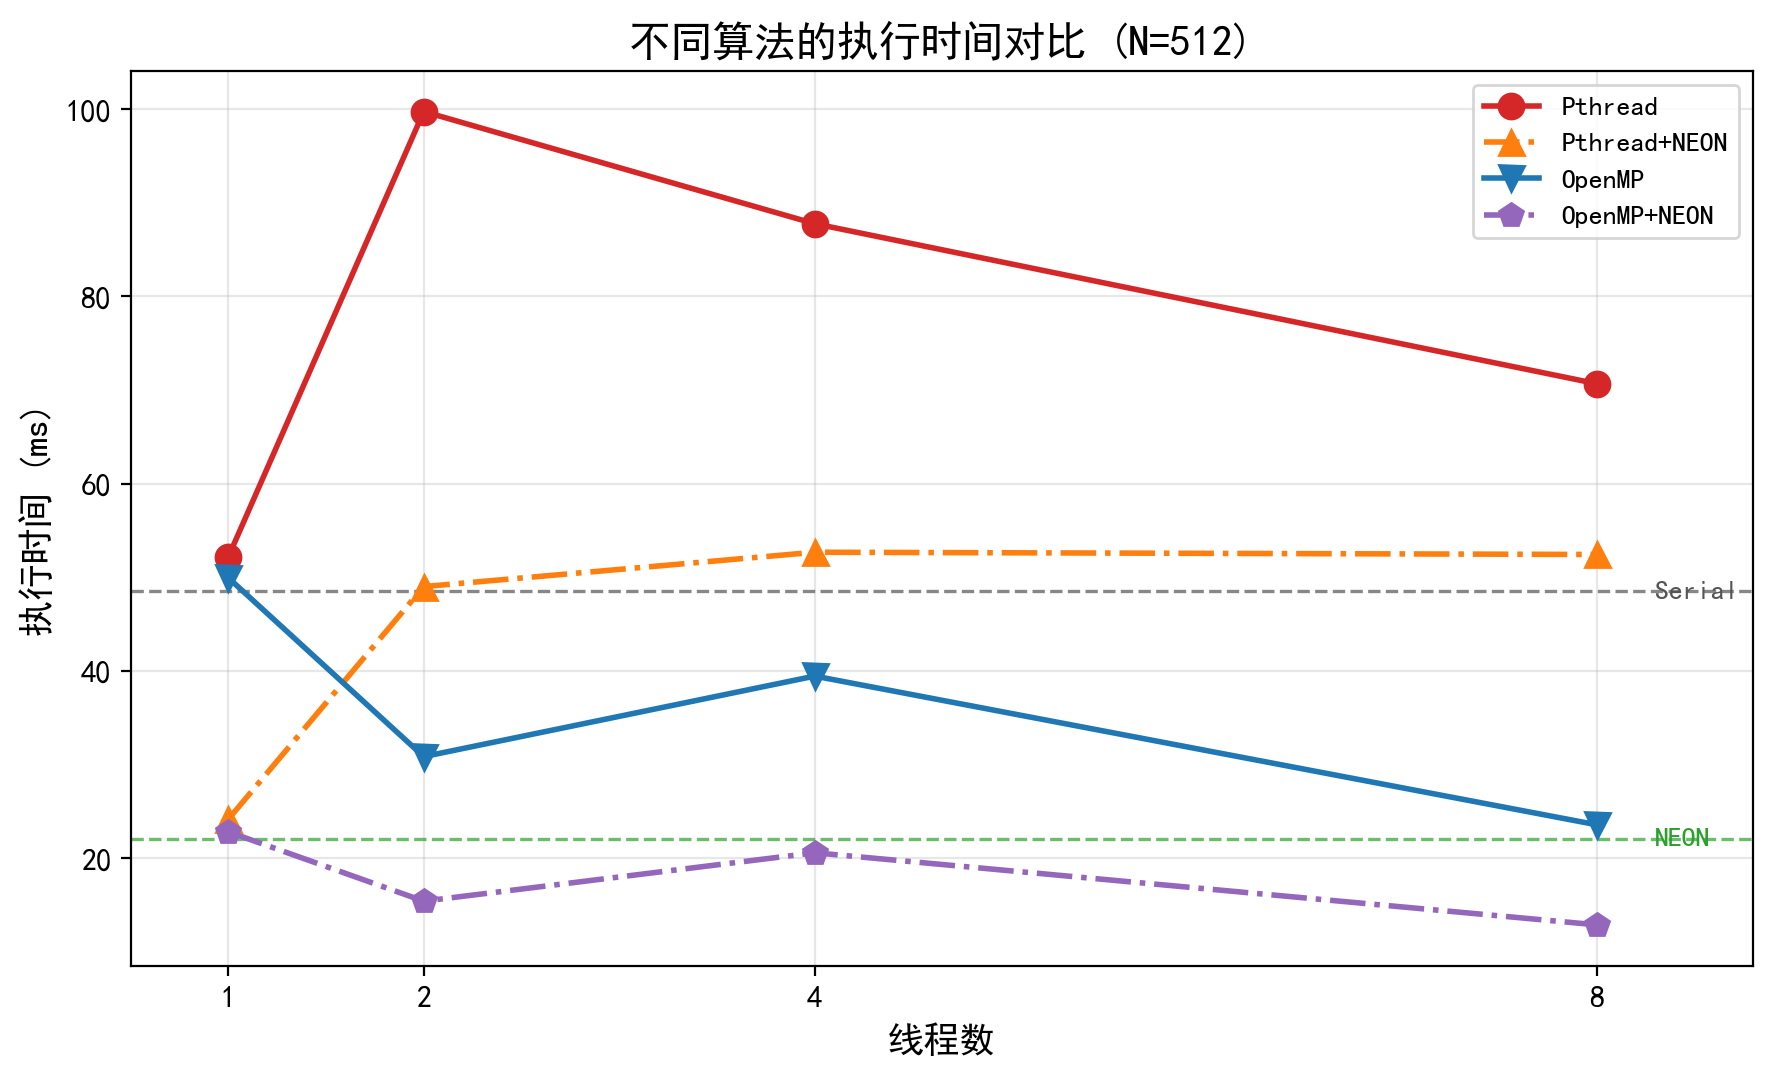
\includegraphics[width=0.48\textwidth]{time_N512.png}}
    \subfigure[N=1024]{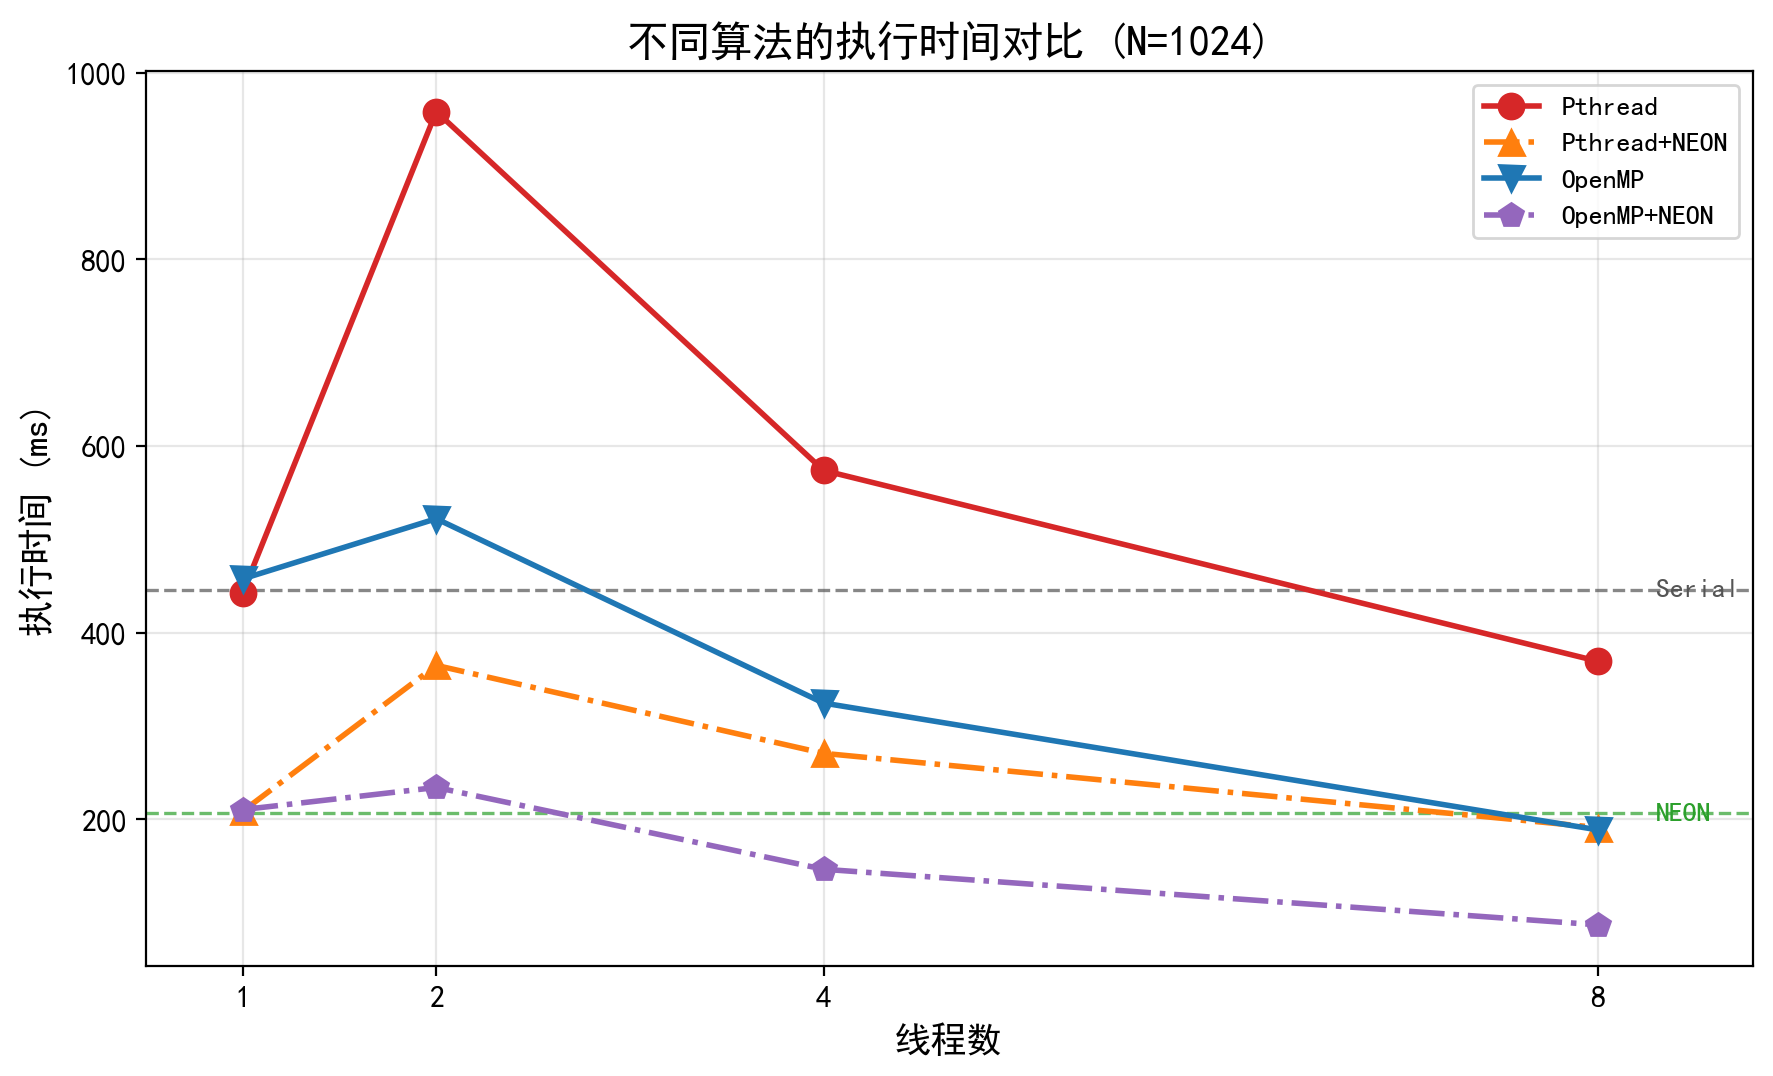
\includegraphics[width=0.48\textwidth]{time_N1024.png}}
    \subfigure[N=2048]{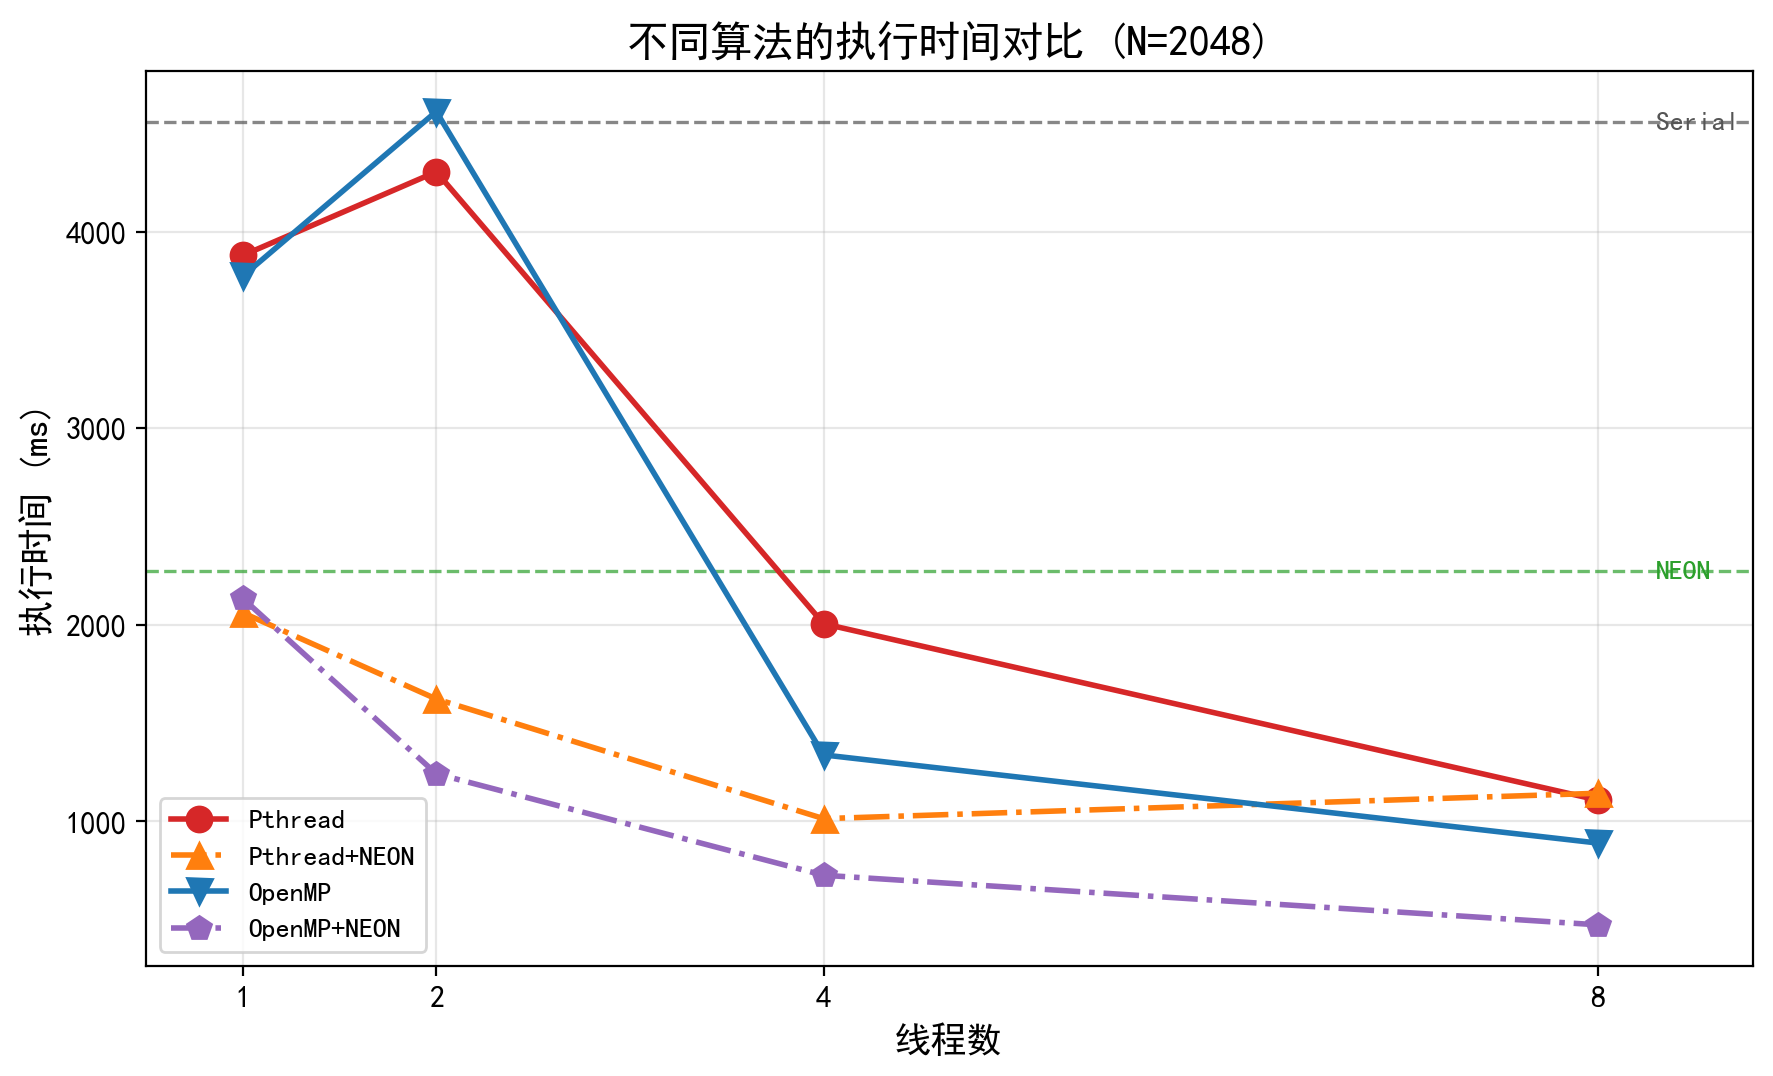
\includegraphics[width=0.48\textwidth]{time_N2048.png}}
    \caption{各算法执行时间随线程数变化}
    \label{fig:time_all}
\end{figure}

\subsection{加速比分析}

表 \ref{table:speedup} 列出了各并行版本在不同配置下的加速比（相对于串行版本）。图 \ref{fig:speedup_all} 直观展示了加速比随线程数的变化趋势。

\begin{table}[H]
  \centering
  \caption{加速比汇总（相对串行）}
  \label{table:speedup}
  \small
  \begin{tabular}{|c|c|c|c|c|c|c|}
  \hline
  N & 线程 & NEON & Pthread & Pth+NEON & OMP & OMP+NEON \\
  \hline
  \multirow{4}{*}{512} & 1 & 2.20x & 0.93x & 2.01x & 0.97x & 2.13x \\
   & 2 & -- & 0.49x & 0.99x & 1.57x & 3.15x \\
   & 4 & -- & 0.55x & 0.92x & 1.23x & 2.36x \\
   & 8 & -- & 0.69x & 0.93x & 2.06x & \textbf{3.77x} \\
  \hline
  \multirow{4}{*}{1024} & 1 & 2.16x & 1.01x & 2.14x & 0.98x & 2.12x \\
   & 2 & -- & 0.47x & 1.22x & 0.85x & 1.91x \\
   & 4 & -- & 0.78x & 1.65x & 1.37x & 3.05x \\
   & 8 & -- & 1.21x & 2.33x & 2.37x & \textbf{5.13x} \\
  \hline
  \multirow{4}{*}{2048} & 1 & 2.01x & 1.17x & 2.21x & 1.21x & 2.13x \\
   & 2 & -- & 1.06x & 2.81x & 0.99x & 3.67x \\
   & 4 & -- & 2.27x & 4.50x & 3.41x & 6.28x \\
   & 8 & -- & 4.12x & 3.99x & 5.13x & \textbf{9.64x} \\
  \hline
  \end{tabular}
\end{table}

\begin{figure}[H]
    \centering
    \subfigure[N=512]{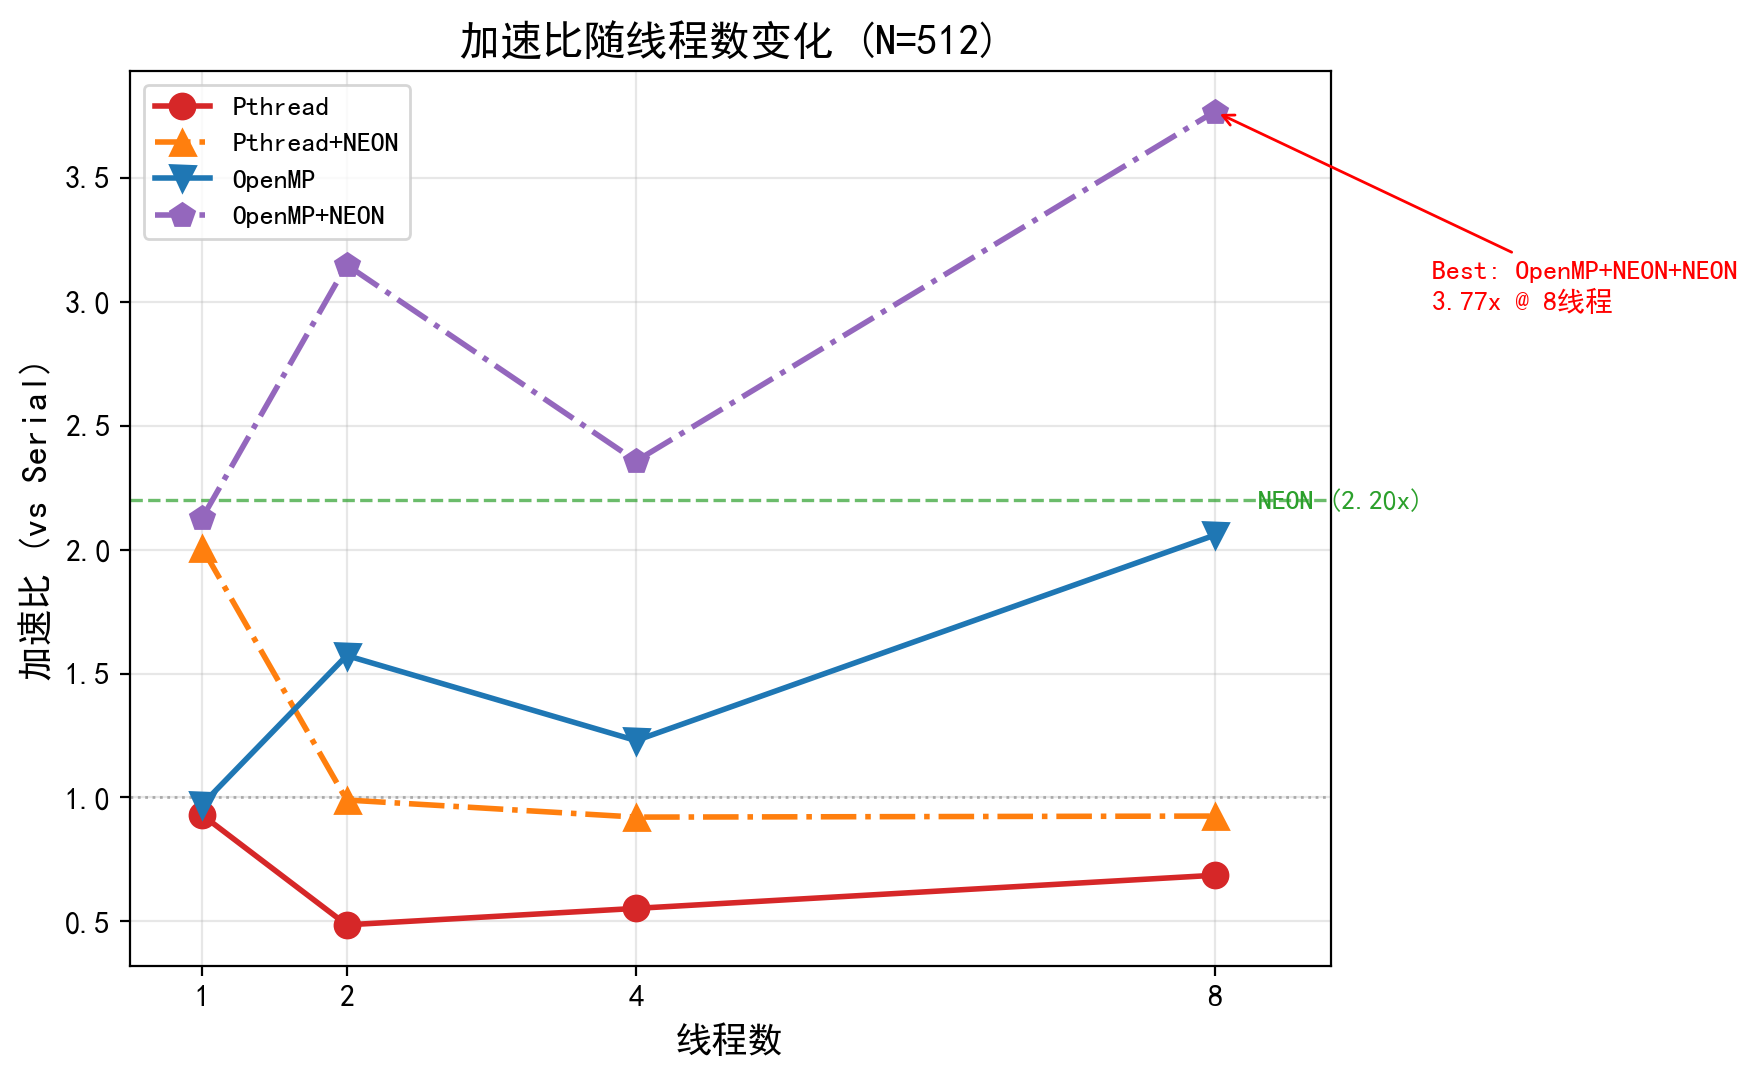
\includegraphics[width=0.48\textwidth]{speedup_N512.png}}
    \subfigure[N=1024]{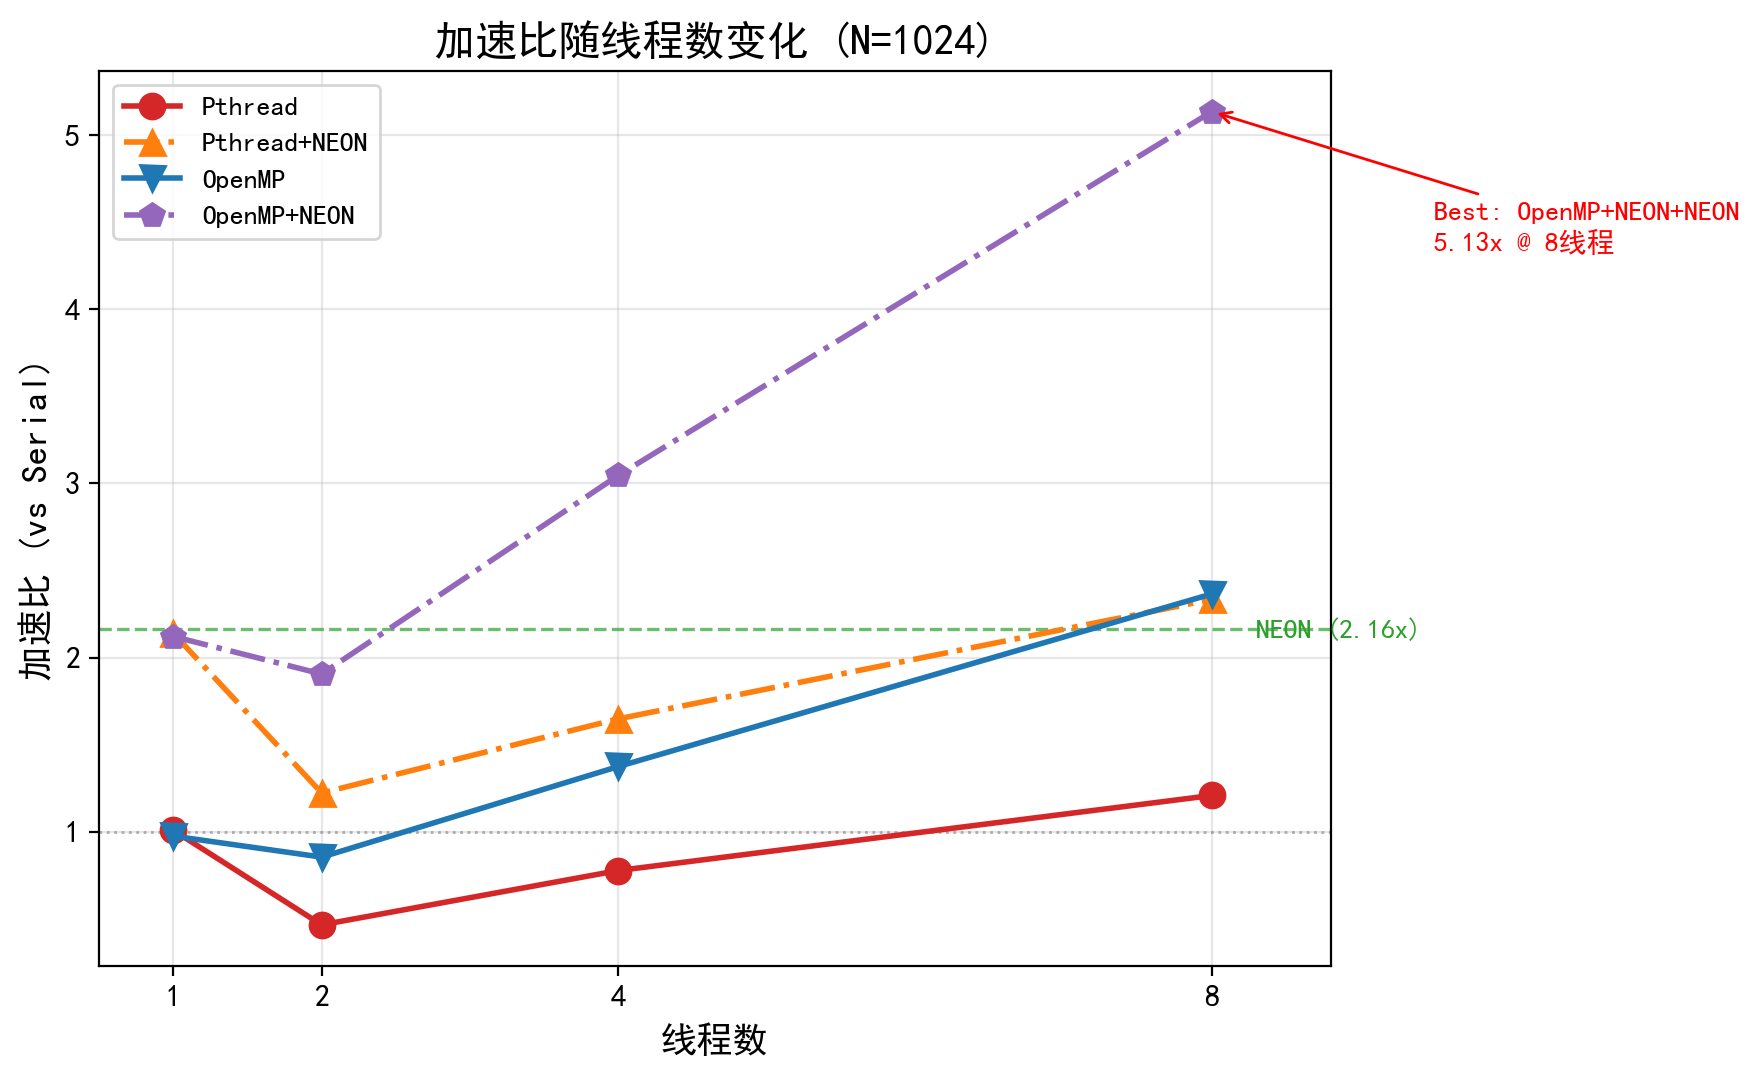
\includegraphics[width=0.48\textwidth]{speedup_N1024.png}}
    \subfigure[N=2048]{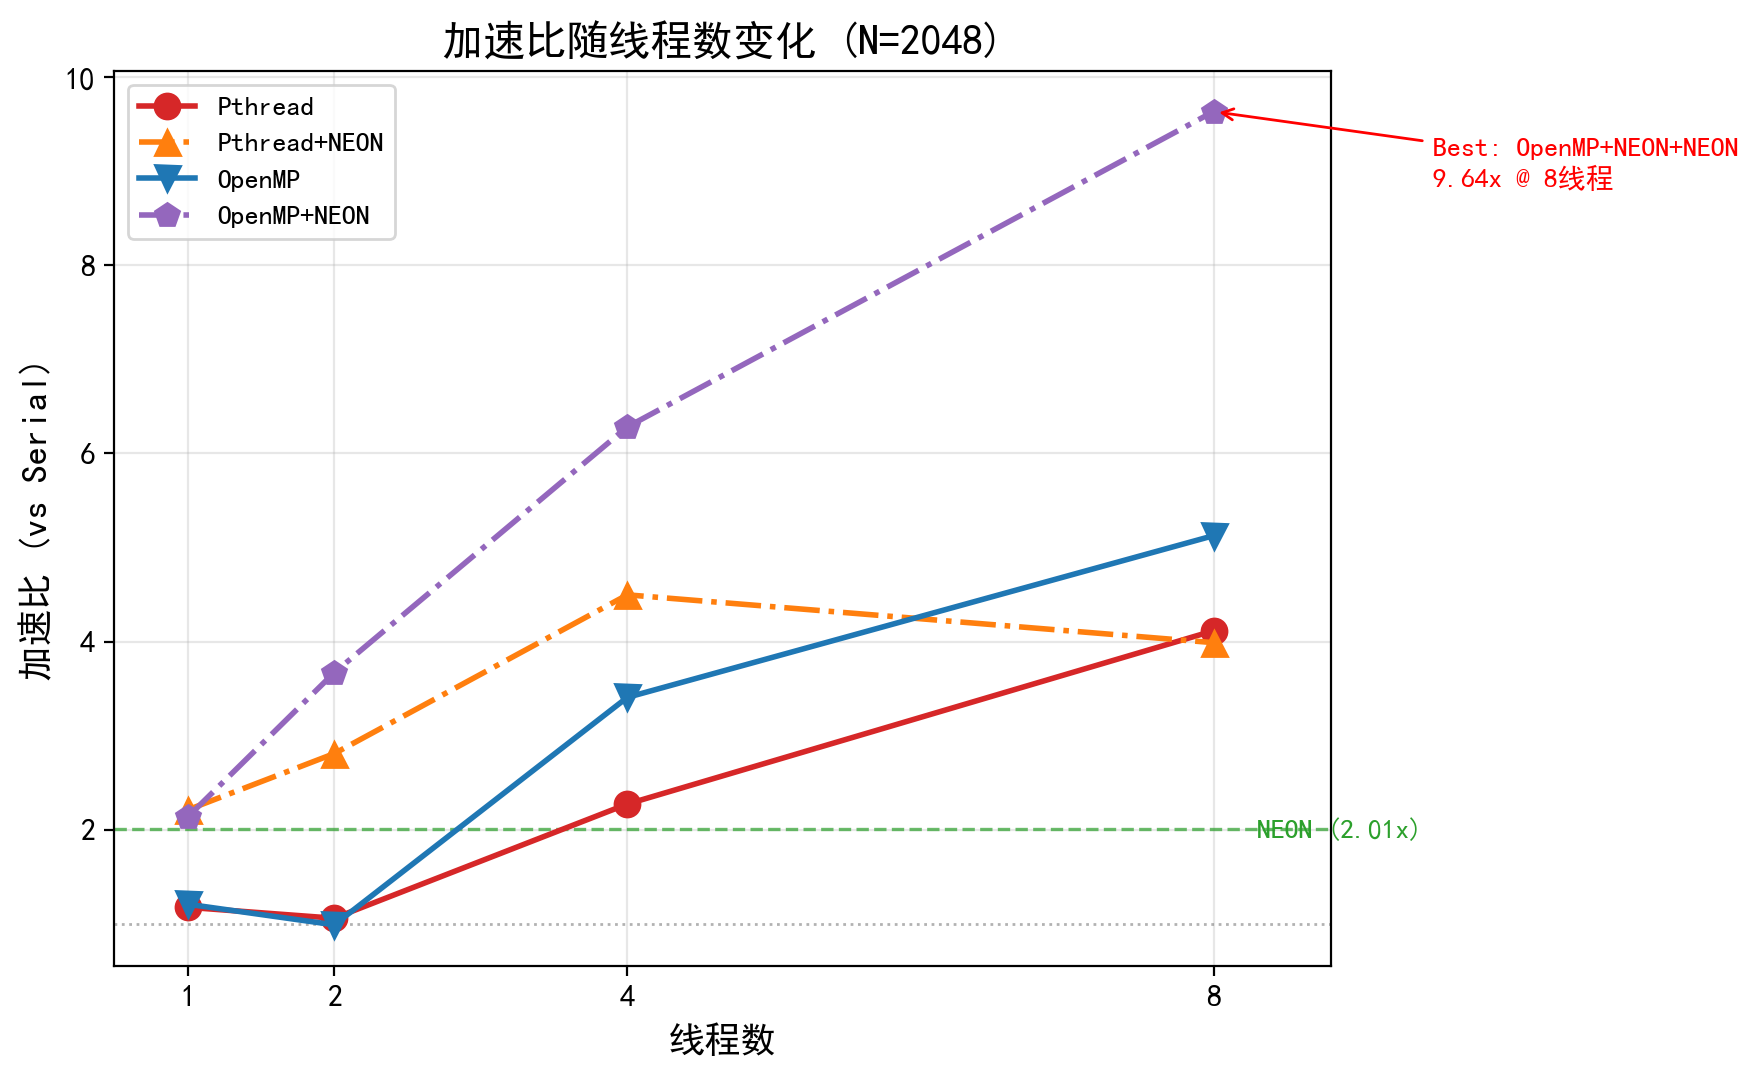
\includegraphics[width=0.48\textwidth]{speedup_N2048.png}}
    \caption{加速比随线程数变化}
    \label{fig:speedup_all}
\end{figure}

\begin{figure}[H]
    \centering
    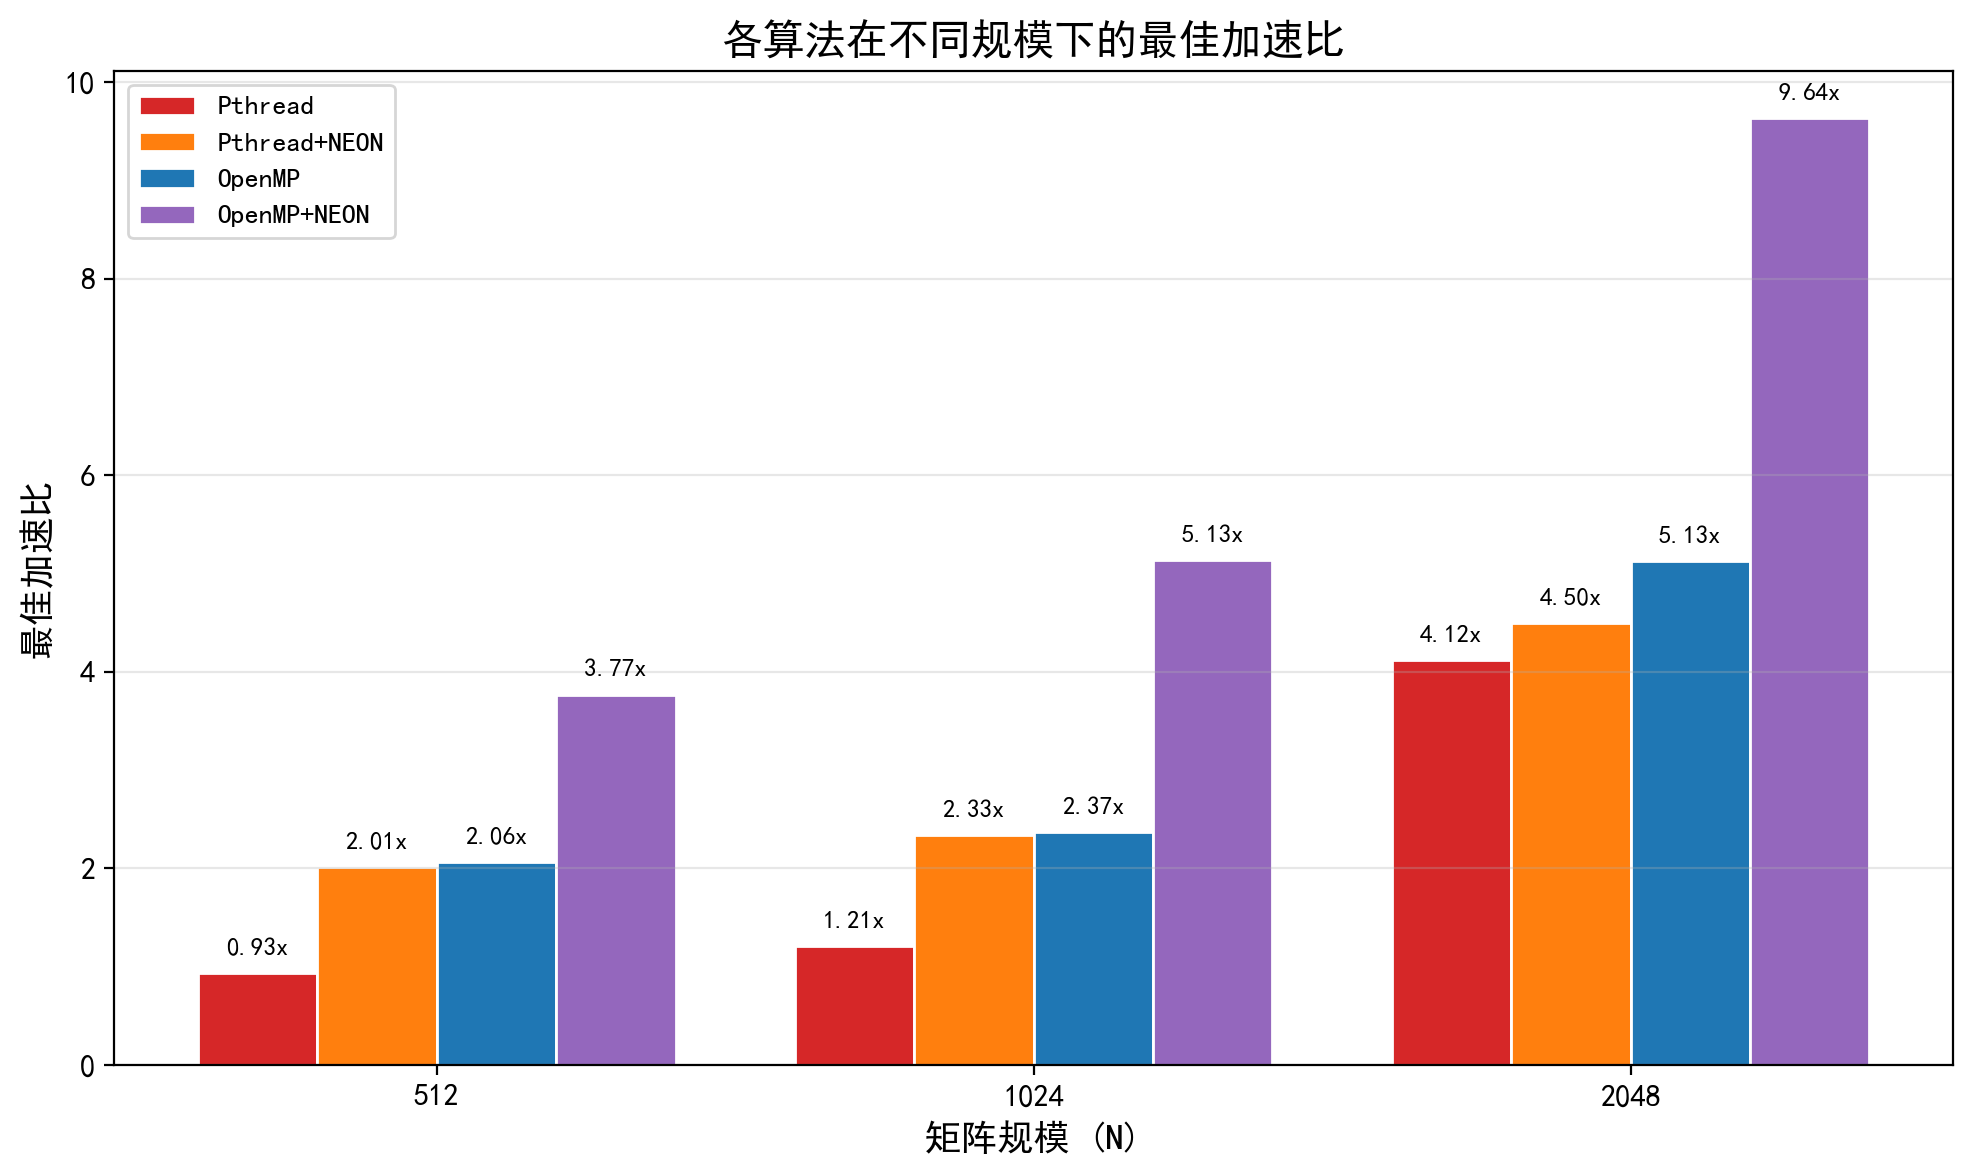
\includegraphics[width=0.75\textwidth]{best_speedup_bar.png}
    \caption{各算法在不同规模下的最佳加速比}
    \label{fig:best_bar}
\end{figure}

\subsection{Pthread 与 OpenMP 性能对比分析}

本节从多个维度对 Pthread 和 OpenMP 两种编程模型进行系统对比。

\subsubsection{编程复杂度}

Pthread 版本需要手动管理线程生命周期（\texttt{pthread\_create / pthread\_join}）、设计参数传递结构体（\texttt{ThreadParam}）、初始化与销毁 barrier（\texttt{pthread\_barrier\_init / destroy}）以及手写循环划分逻辑。OpenMP 版本仅需在串行代码上添加 3 条 \texttt{\#pragma} 编译制导指令，代码量约为 Pthread 版本的 1/3。从工程角度看，OpenMP 的声明式并行模型显著降低了多线程编程的入门门槛和维护成本。

\subsubsection{线程管理开销}

实验数据显示，Pthread 版本在 N=512/1024 且线程数为 2 时出现了严重的性能劣化（加速比仅 0.47x--0.49x），而 OpenMP 同等条件下的加速比为 0.85x--1.57x。这一差异的根源在于：

\begin{itemize}
    \item Pthread 的 \texttt{pthread\_barrier\_wait} 涉及内核态切换，在 N=1024 时需要 2048 次（$2 \times 1024$）barrier 同步，每次同步开销约 0.2--0.5ms，总计同步开销可达 400--1000ms，远超小规模下的实际计算时间。
    \item OpenMP 的隐式 barrier（\texttt{\#pragma omp single} 和 \texttt{\#pragma omp for} 自带）由运行时优化，可能使用用户态自旋等待（spin-wait）减少内核切换。
    \item OpenMP 运行时使用\textbf{线程池}技术，线程在 \texttt{parallel} 区域结束后并不销毁，而是返回线程池等待下次复用。这与 Pthread 静态线程池范式在概念上相似，但 OpenMP 的线程池实现在调度和唤醒延迟上更为优化。
\end{itemize}

\subsubsection{调度机制}

Pthread 版本采用手工循环划分（静态分配），每个线程在每轮消去中处理的行的集合是确定的。OpenMP 版本使用 \texttt{schedule(dynamic, 16)} 动态调度——线程完成当前 16 行的任务块后，运行时自动分配下一个 16 行的任务块。动态调度的优势在 N=2048 时显现：每轮消去中各行计算量差异明显（越靠后的行需要消去的列越多），动态调度让快线程自动承接更多工作，减少线程空闲等待。

\subsubsection{运行效率}

图 \ref{fig:efficiency} 展示了各算法的并行效率（加速比/线程数）。理想情况下效率 = 1.0，表示线性加速。N=2048 时 OpenMP+NEON 在 8 线程下达到 1.20 的效率（超线性加速），这得益于多核 Cache 的聚合效应——8 个核的 L1 Cache 总容量是单核的 8 倍，部分工作集可以容纳在聚合 Cache 中。

\begin{figure}[H]
    \centering
    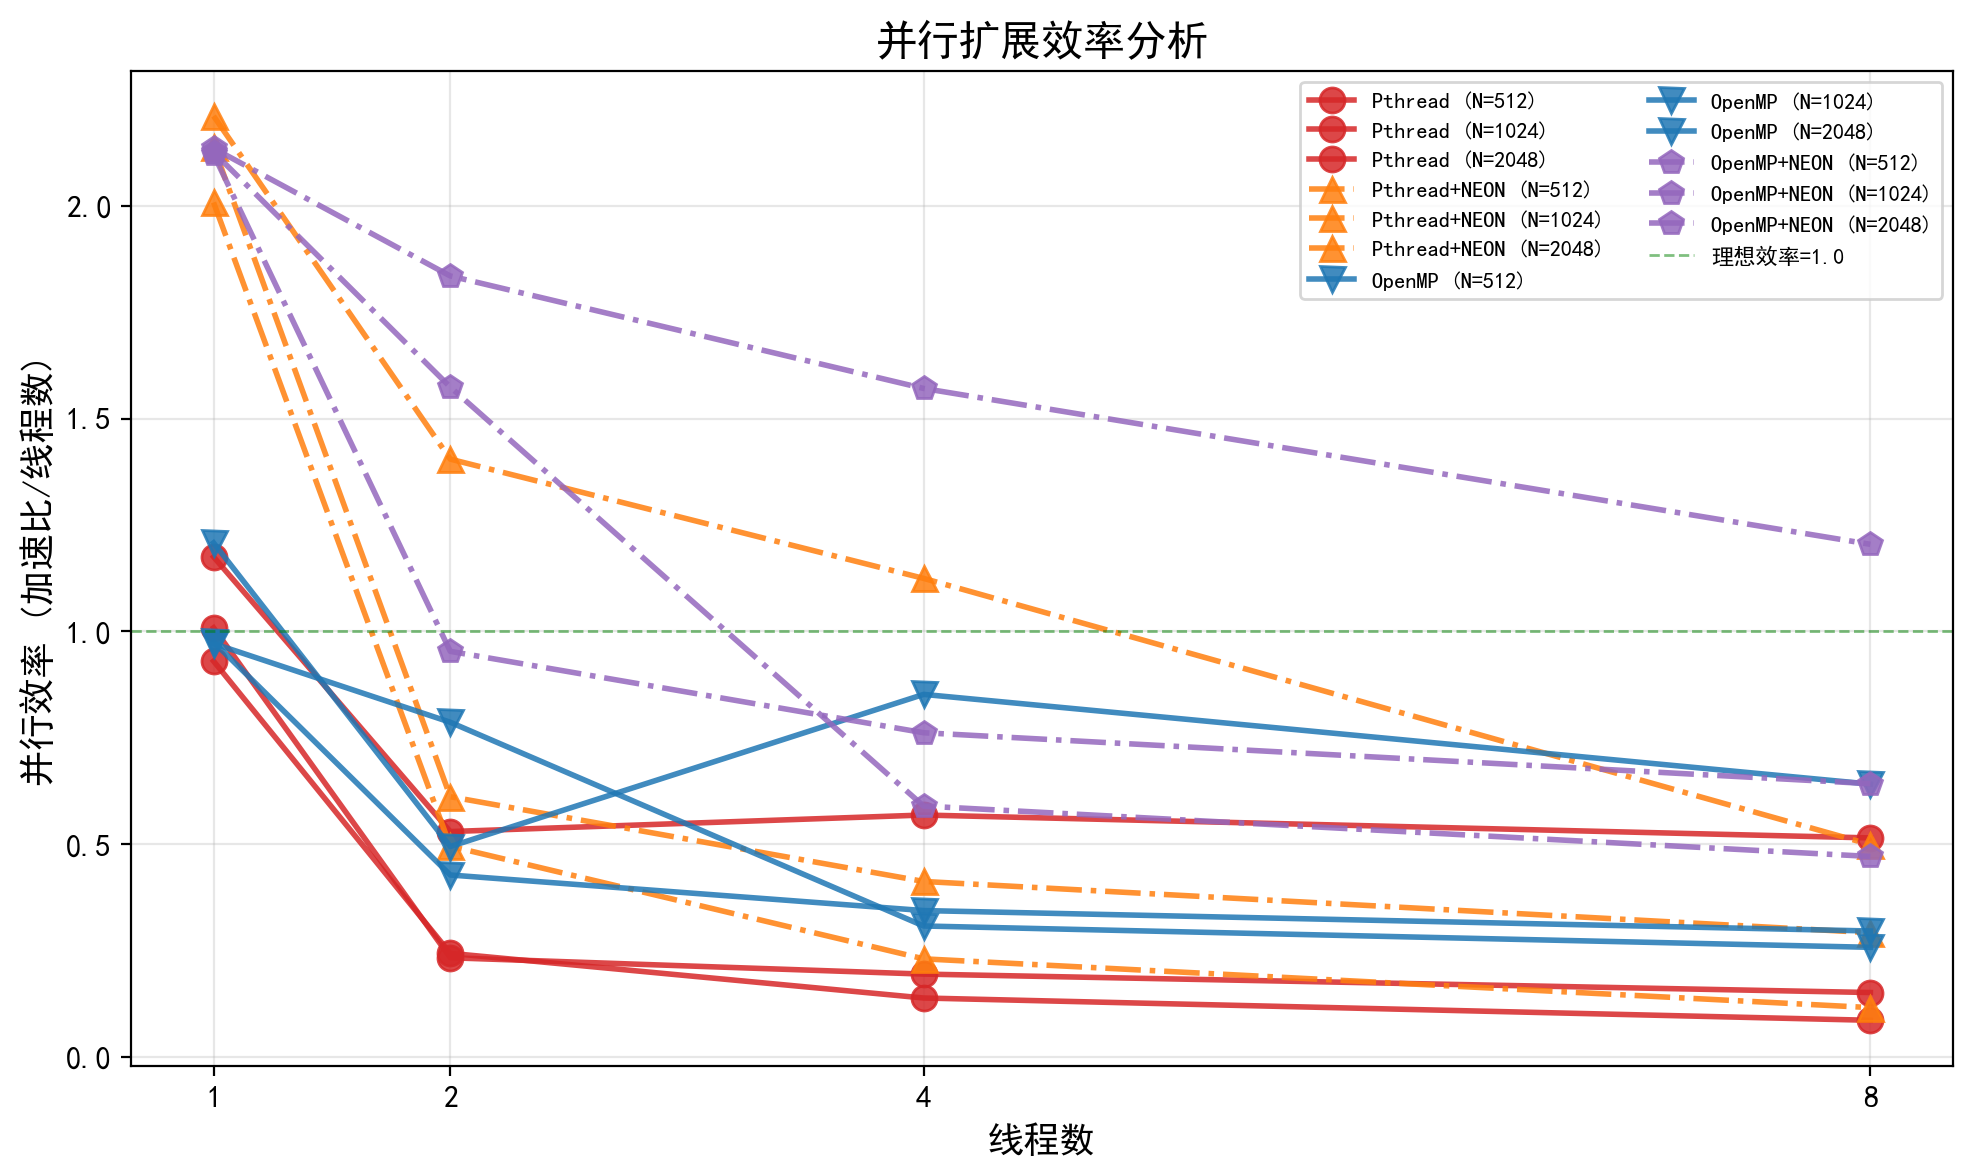
\includegraphics[width=0.75\textwidth]{efficiency.png}
    \caption{并行效率分析（加速比/线程数）}
    \label{fig:efficiency}
\end{figure}

\subsection{规模扩展性分析}

从图 \ref{fig:speedup_all} 和表 \ref{table:speedup} 可以总结出以下扩展性规律：

\begin{enumerate}
    \item \textbf{小规模（N=512）：} 计算量不足以掩盖线程同步开销。Pthread 所有线程数下加速比均 < 1.0（负优化），最佳方案是纯 NEON（2.20x）而非多线程。
    \item \textbf{中规模（N=1024）：} 4--8 线程开始产生正收益。OpenMP+NEON 在 8 线程达到 5.13x，Pthread+NEON 在 8 线程达到 2.33x。
    \item \textbf{大规模（N=2048）：} 计算密度足够高，多线程收益最大化。OpenMP+NEON 达到 9.64x，OpenMP 标量达到 5.13x，Pthread 标量达到 4.12x。加速比增长趋势表明，若有更多核心可用，加速比仍有进一步提升的空间。
\end{enumerate}

图 \ref{fig:overview} 汇总了所有测试组合的加速比，进一步印证了上述分析。

\begin{figure}[H]
    \centering
    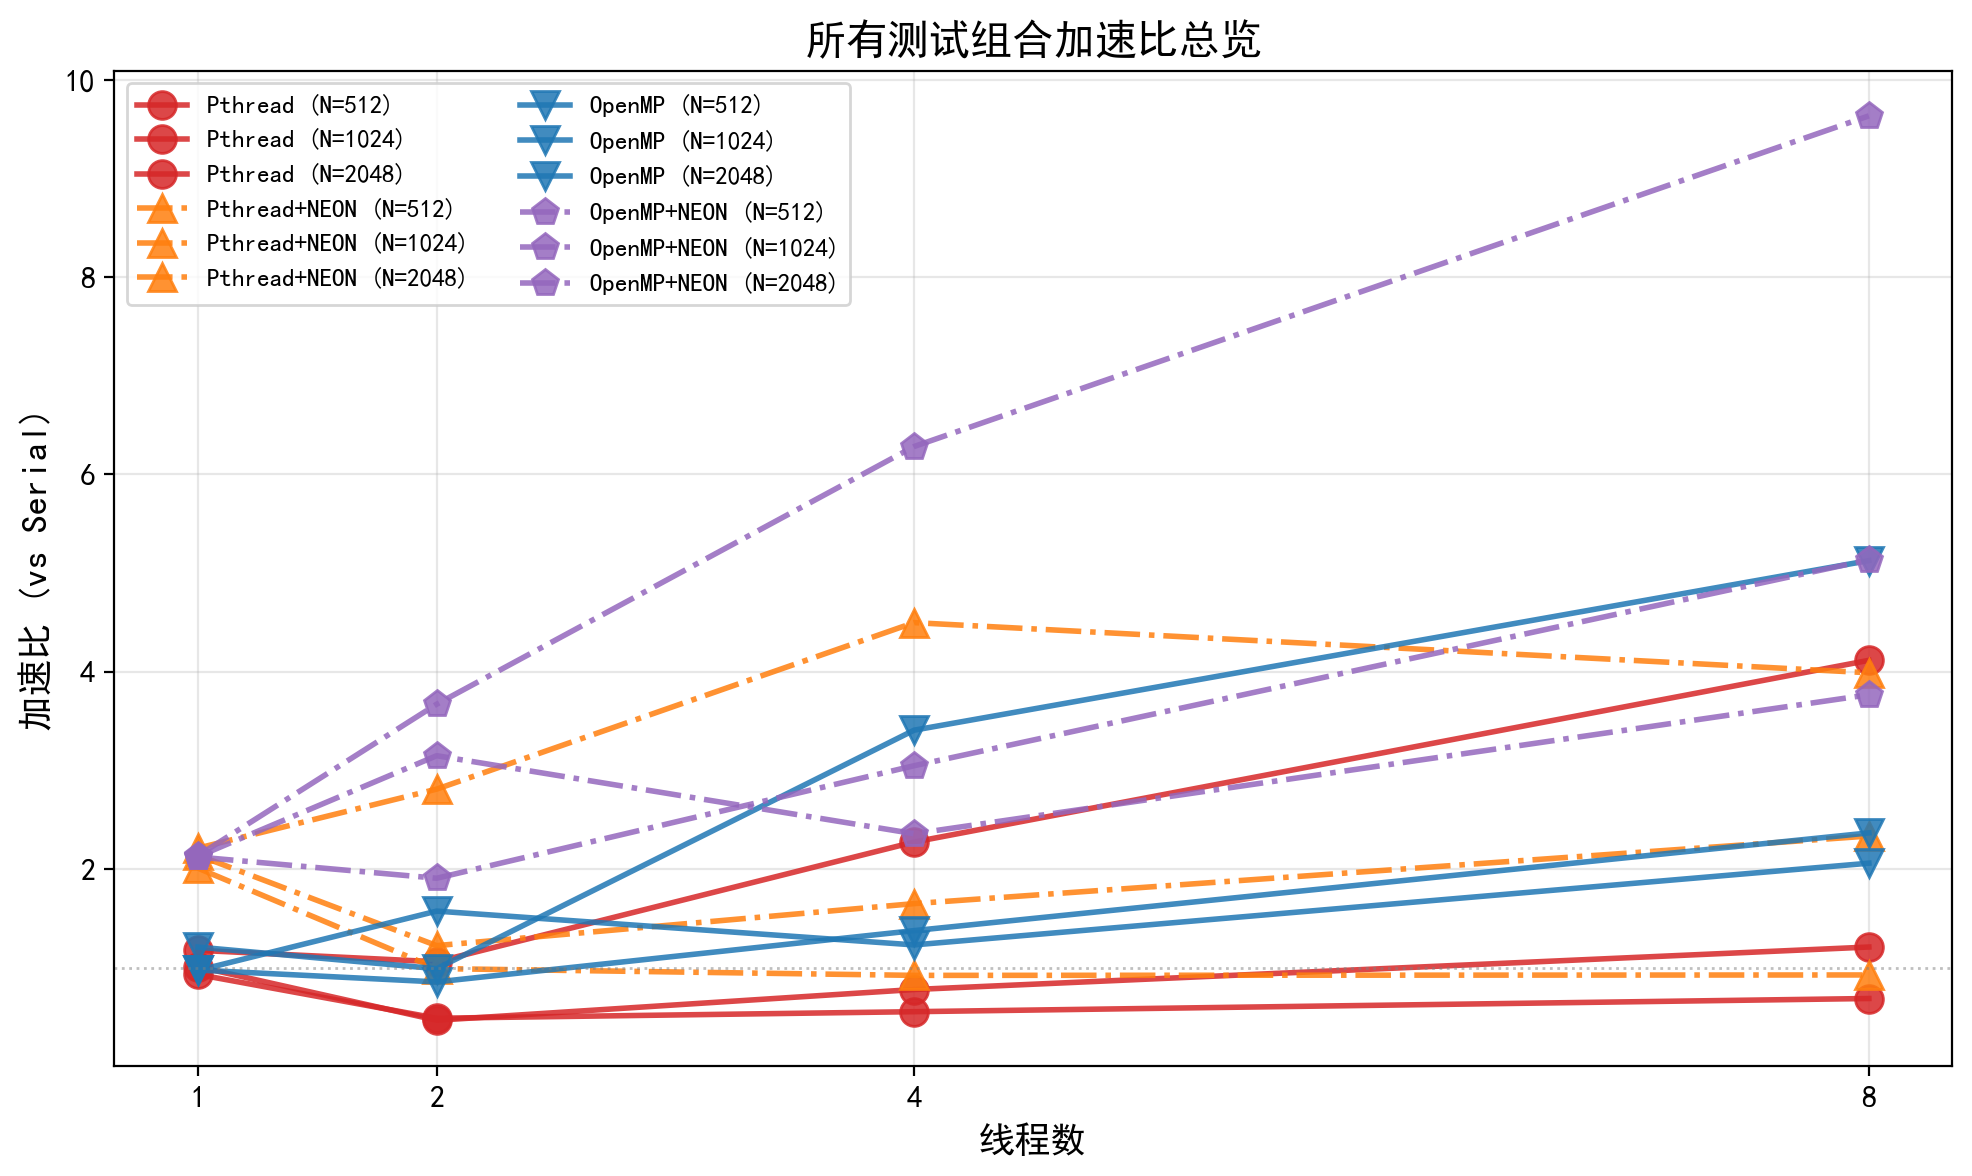
\includegraphics[width=0.85\textwidth]{speedup_overview.png}
    \caption{全部测试组合加速比总览}
    \label{fig:overview}
\end{figure}

\subsection{任务划分策略与同步机制讨论}

\subsubsection{行划分（水平划分）}

本实验采用的行划分策略将消去循环的外层（$i$ 循环）拆分给各线程。这是高斯消去最自然的并行方式——每行消去计算互相独立，无需临界区保护。缺点在于：随着 $k$ 增大，每行的计算量递减（需要处理的 $j$ 列越来越少），静态分配时后分配的行计算量更少，可能造成负载不均。循环划分和动态调度均在一定程度上缓解了此问题。

\subsubsection{列划分（垂直划分）的考量}

列划分将消去循环的内层（$j$ 循环）拆分，每个线程负责消去行的一部分列。列划分的优点是在每轮消去中各线程的计算量完全均匀，但需要额外的同步——因为 NEON 向量化要求连续访存，列划分会将连续内存打散到不同线程，可能导致 Cache Line 伪共享（False Sharing），反而降低性能。由于 ARM AArch64 架构对连续访存高度优化，行划分配合 NEON 连续加载是最优选择。

\subsubsection{同步机制}

Barrier 同步是高斯消去并行化的核心挑战。每轮消去需要两次同步（归一化后、消去后），N 轮共计 $2N$ 次同步。Pthread barrier 和 OpenMP 隐式 barrier 的性能差异直接决定了小规模下的总体性能。在大规模（N=2048）下，单轮计算时间 >> 同步时间，同步开销被有效摊薄。

\subsection{体系结构相关优化分析}

\subsubsection{Cache 利用}

N=2048 时矩阵占用 16MB（$2048^2 \times 4$ 字节），远超鲲鹏 920 的 L2 Cache（通常 512KB--1MB/core）。然而，高斯消去的计算模式具有天然的 Cache 友好性：第 $k$ 行在归一化后被所有消去线程频繁读取（只读），该行数据会被各核的 L1 Cache 缓存，从而实现高效的 Cache 共享。OpenMP+NEON 在 8 线程下达到超线性加速（效率 > 1.0），印证了多核聚合 Cache 的收益。

\subsubsection{内存对齐}

通过 \texttt{posix\_memalign} 确保每行 16 字节对齐，使得 NEON 向量加载指令 \texttt{vld1q\_f32} 能在单次访存中获取完整的 128 位数据，避免跨 Cache Line 加载的额外开销。

\section{总结}

本次实验在 ARM 鲲鹏 920 平台上系统实现了 Pthread 和 OpenMP 两种多线程模型加速的高斯消去算法，共 6 个算法版本。通过对 3 个矩阵规模 × 4 个线程数的全组合测试，得出以下主要结论：

\begin{enumerate}
    \item \textbf{NEON 向量化是稳定基础：} 在所有规模下纯 NEON 均提供约 2.0x--2.2x 的稳定加速比，与 Lab2 结论一致。
    \item \textbf{最佳组合为 OpenMP+NEON：} 在 N=2048、8 线程时达到 9.64x 加速比，相比纯 NEON 提升约 4.8 倍，相比串行算法提升近 10 倍。
    \item \textbf{OpenMP 整体优于 Pthread：} OpenMP 的线程池机制、用户态自旋等待和动态调度在编程复杂度、小规模性能和扩展性方面均优于手工 Pthread barrier 方案。
    \item \textbf{小规模不宜多线程：} N=512 时线程同步开销超过计算收益，纯 NEON（2.20x）是最佳选择。
    \item \textbf{同步开销是多线程的首要瓶颈：} N=1024 时 2048 次 barrier 同步开销可达数百毫秒，Pthread 在 2 线程下加速比仅 0.47x。
\end{enumerate}

未来工作可以探索更多优化方向：使用 \texttt{schedule(guided)} 替代 \texttt{schedule(dynamic)} 进一步降低调度开销；尝试列划分与行划分的混合策略；引入 perf 工具进行 Cache Miss 和分支预测的深入 profiling 分析。

%============================ 附录 ============================
\newpage
\section*{附录：Git 项目链接}
本实验的完整源代码及提交记录已托管至 Git 平台，项目仓库地址如下：\\
\url{https://github.com/NKU025/Parallel-Gaussian-Elimination}

% 参考文献
\renewcommand{\refname}{参考文献}
\begin{thebibliography}{99}

\bibitem{quinn}
Michael J. Quinn.
\textit{Parallel Programming in C with MPI and OpenMP} [M].
McGraw-Hill, 2004.

\bibitem{golub}
Gene H. Golub and Charles F. Van Loan.
\textit{Matrix Computations, 4th Edition} [M].
Johns Hopkins University Press, 2013.

\bibitem{arm_neon}
ARM Developer.
\textit{Neon Intrinsics Reference} [EB/OL].
\url{https://developer.arm.com/architectures/instruction-sets/intrinsics/}

\bibitem{openmp}
OpenMP Architecture Review Board.
\textit{OpenMP Application Programming Interface Version 4.5} [EB/OL].
\url{https://www.openmp.org/}

\end{thebibliography}

\end{document}
